\documentclass[pdflatex,sn-vancouver-num]{sn-jnl}

\usepackage{graphicx}
\usepackage{amsmath,amssymb,amsfonts}
\usepackage{booktabs}
\usepackage{xcolor}

\graphicspath{{./}{results/figures/}}
\raggedbottom

% Numbers of the main article's sections and tables referred to below (checked against the compiled article).
\newcommand{\MainSecLowVolume}{6.6}
\newcommand{\MainSecMechanism}{7}
\newcommand{\MainTabAblation}{5}
\newcommand{\MainTabProtocol}{6}
\newcommand{\MainTabKaggle}{7}
\newcommand{\MainTabLowVolume}{4}
\newcommand{\MainRefNadeau}{48}
\newcommand{\MainRefBouckaert}{49}

\renewcommand{\thetable}{S\arabic{table}}
\renewcommand{\thefigure}{S\arabic{figure}}
\renewcommand{\thesection}{S\arabic{section}}

\begin{document}

\title[Online Resource 1]{Online Resource 1 for ``When Does Relational Structure Help Healthcare Fraud
Detection? A Controlled Benchmark of Heterogeneous Graph Neural Networks and Graph-Augmented Tabular
Models'', \textit{Health Information Science and Systems}}

\author*[1]{\fnm{H M} \sur{Akshay}}\email{rvit23bcs106.rvitm@rvei.edu.in}
\author[1]{\fnm{Gaurav} \sur{S B}}\email{rvit23bcs258.rvitm@rvei.edu.in}
\author[1]{\fnm{Eshita} \sur{Narayana}}\email{rvit23bcs031.rvitm@rvei.edu.in}
\author[1]{\fnm{Harshita} \sur{Srivastava}}\email{rvit23bcs323.rvitm@rvei.edu.in}
\author[1]{\fnm{Malini M} \sur{Patil}}\email{malinimp.rvitm@rvei.edu.in}

\affil[1]{\orgdiv{Department of Computer Science and Engineering},
\orgname{RV Institute of Technology and Management},
\orgaddress{\city{Bengaluru}, \postcode{560083}, \state{Karnataka}, \country{India}}}

\abstract{This Online Resource accompanies the article named in the title. It contains material summarised
but not shown in full there: the selected hyperparameters, the two-stage routing evaluation, the ring-volume
dose-response, the confirmatory test of the hybrid result, the cost of training and scoring, single-factor
ablations of HGT, which inputs the trained models use, figures of the mechanism ablations and of new versus
recurring rings, repeated cross-validation and per-rotation tuning on the public data, and a re-analysis of a
small fixed benchmark. Every number is generated from the run records in the article's code repository.}

\maketitle

\section{Selected hyperparameters}\label{sec:s_hyper}
Table~\ref{tab:hyperparams} lists the configurations selected with the equal tuning budget.

\begin{table}[h]
\caption{Selected hyperparameters (equal budget per method; hybrids inherit their base configuration; methods sharing a search space were offered the same candidate configurations). Synthetic: tuned on development worlds; public data: tuned on a separate split. The configurations re-tuned for the low-volume stress test are in the repository (\texttt{results/tuning\_lowvolume}).}\label{tab:hyperparams}
\scriptsize
\begin{tabular}{@{}p{2.2cm}p{5.0cm}p{5.0cm}@{}}
\toprule
Method & Synthetic benchmark & Public data \\
\midrule
LR & C=100 & C=1 \\
RF & max depth=16; max features=sqrt; min samples leaf=3; n estimators=300 & max depth=16; max features=0.3; min samples leaf=10; n estimators=300 \\
GB (C) & l2=0; learning rate=0.03; max iter=200; max leaf nodes=15; min samples leaf=10 & -- \\
GB (C+A / P) & l2=1; learning rate=0.1; max iter=200; max leaf nodes=63; min samples leaf=50 & l2=0; learning rate=0.03; max iter=200; max leaf nodes=15; min samples leaf=50 \\
GB (C+A+G / P+G) & l2=1; learning rate=0.1; max iter=400; max leaf nodes=15; min samples leaf=20 & l2=0; learning rate=0.03; max iter=200; max leaf nodes=15; min samples leaf=50 \\
GB (P+G+L) & -- & l2=0; learning rate=0.03; max iter=200; max leaf nodes=15; min samples leaf=50 \\
MLP & dropout=0.3; hidden=128; layers=2; lr=0.001; weight decay=1e-05 & dropout=0.3; hidden=128; layers=2; lr=0.001; weight decay=1e-05 \\
SAGE & aggr=sum; dropout=0.1; hidden=32; layers=3; lr=0.003; weight decay=0.001 & aggr=mean; dropout=0.3; hidden=64; layers=3; lr=0.003; weight decay=0.0001 \\
RGCN & aggr=sum; dropout=0.3; hidden=64; layers=2; lr=0.003; weight decay=0.001 & aggr=sum; dropout=0.3; hidden=64; layers=2; lr=0.01; weight decay=0.001 \\
HAN & dropout=0.3; heads=4; hidden=32; layers=3; lr=0.01; weight decay=1e-05 & dropout=0.1; heads=2; hidden=64; layers=2; lr=0.003; weight decay=0.0001 \\
Simple-HGN & dropout=0.3; heads=4; hidden=64; layers=3; lr=0.003; weight decay=0.0001 & dropout=0.1; heads=4; hidden=64; layers=2; lr=0.01; weight decay=0.001 \\
HGT & dropout=0.3; heads=4; hidden=32; layers=3; lr=0.01; weight decay=1e-05 & dropout=0.1; heads=4; hidden=64; layers=2; lr=0.01; weight decay=0.001 \\
\botrule
\end{tabular}
\end{table}

\section{Two-stage routing}\label{sec:s_routing}

\subsection{Method}\label{sec:s_routing_method}
A common deployment proposal is to score every claim with a cheap tabular
model and pass only high-risk claims to a GNN. We evaluate this with GB-CAG
as the first stage and HGT or SAGE as the second. A claim is escalated if its
GB-CAG score is at least the $(1-e)$ quantile of the GB-CAG scores in the
validation period. The escalation fraction $e\in\{0.05, 0.1, 0.2, 0.3, 0.5,
1\}$ is chosen by validation AP, so test claims never influence it. Escalated
claims rank above all other claims and are ordered either by the GNN score
alone (\emph{re-rank}: GB-CAG acts as a filter) or by the mean of the two
models' validation percentiles (\emph{fused}); non-escalated claims keep
their GB-CAG order. With $e=1$, re-ranking reduces to the GNN alone and
fusion to a rank-average ensemble of the two models, so both single models
and the ensemble are among the candidates. A claim's routed score depends
only on its own two scores and on validation statistics. The stages are the
models of the main experiment, retrained with the same seeds; their test
predictions reproduce the stored ones exactly for the GNNs and to within
$3\times10^{-8}$ for GB-CAG (float32 storage).

\subsection{Results}\label{sec:s_routing_results}
Table~\ref{tab:cascade} and Fig.~\ref{fig:cascade} evaluate two-stage
routing (Section~\ref{sec:s_routing_method}) on the same test claims as the single
models. In the design usually proposed, GB-CAG filters and the GNN decides
(re-rank). Validation mostly selected small escalation fractions (5\% in 30
of 54 worlds for HGT), and the routed system matched GB-CAG (GB-CAG$\to$HGT
$\Delta\text{AP}=-0.001$, 95\% CI $[-0.006, 0.003]$; GB-CAG$\to$SAGE
$+0.001$). Escalating more claims to HGT lowered both ring AP (from 0.980 at
5\% to 0.968 when every claim is escalated) and, more steeply, isolated AP
(from 0.626 to 0.508; Fig.~\ref{fig:cascade}b--d), because HGT ranks both
less well than GB-CAG. Ordering escalated claims by the mean of the two models' percentiles
did better: GB-CAG$\to$HGT gained $+0.003$ (Holm $p=0.60$) and
GB-CAG$\to$SAGE $+0.006$ $[0.003, 0.010]$ (Holm $p=0.042$, positive for all
six seeds), on ring ($+0.006$) and isolated fraud ($+0.023$) alike. Validation, however, chose to fuse
\emph{every} claim in 22 (HGT) and 30 (SAGE) of the 54 worlds, and on average
55\% and 70\% of test claims were escalated: the gain comes from combining two
different rankings, not from routing a subset of claims. The feature-level
hybrids, which give the GNN the engineered features, had slightly higher
ring AP ($+0.008$, not significant with the seed as unit) but lost
0.08--0.11 isolated AP and so matched GB-CAG overall. At the ring level all
methods reached the ceiling: in all 54 worlds each test ring had at least one
claim among the top 5\% of claims, and precision in that budget was
0.989--0.998 for every method.

\begin{table}[h]
\caption{Two-stage routing versus single models and feature-level hybrids, averaged over the 54 worlds (same test claims for every row). Routing escalates claims whose GB-CAG score exceeds a threshold set on validation data; the escalation fraction is chosen by validation AP. P@5\%: precision among the top 5\% of test claims. Esc.: mean share of test claims escalated. $\Delta$AP: paired difference in AP from GB-CAG ($\pm$ half-width of the 95\% $t$-interval over the six generator seeds), Holm-adjusted $p$ over the rows.}\label{tab:cascade}
\scriptsize
\setlength{\tabcolsep}{2.5pt}
\begin{tabular}{@{}lcccccc@{}}
\toprule
Method & AP & Ring AP & Isol.\ AP & P@5\% & Esc. & $\Delta$AP ($p$) \\
\midrule
GB-CAG & 0.947 & 0.979 & 0.626 & 0.996 & -- & -- \\
HGT & 0.929 & 0.968 & 0.507 & 0.989 & -- & $-0.018$ $\pm$ 0.013 (0.104) \\
SAGE & 0.940 & 0.979 & 0.541 & 0.995 & -- & $-0.007$ $\pm$ 0.009 (0.597) \\
\midrule
HGT+AG & 0.945 & 0.986 & 0.514 & 0.996 & -- & $-0.002$ $\pm$ 0.006 (1.000) \\
SAGE+AG & 0.947 & 0.987 & 0.548 & 0.996 & -- & $0.000$ $\pm$ 0.005 (1.000) \\
\midrule
GB-CAG$\to$HGT, re-rank & 0.945 & 0.979 & 0.606 & 0.995 & 0.16 & $-0.001$ $\pm$ 0.005 (1.000) \\
GB-CAG$\to$HGT, fused & 0.950 & 0.981 & 0.640 & 0.997 & 0.55 & $+0.003$ $\pm$ 0.004 (0.597) \\
GB-CAG$\to$SAGE, re-rank & 0.948 & 0.983 & 0.595 & 0.997 & 0.24 & $+0.001$ $\pm$ 0.004 (1.000) \\
GB-CAG$\to$SAGE, fused & 0.953 & 0.985 & 0.648 & 0.998 & 0.70 & $+0.006$ $\pm$ 0.004 (0.042) \\
\botrule
\end{tabular}
\end{table}

\begin{figure}[t]
\centering
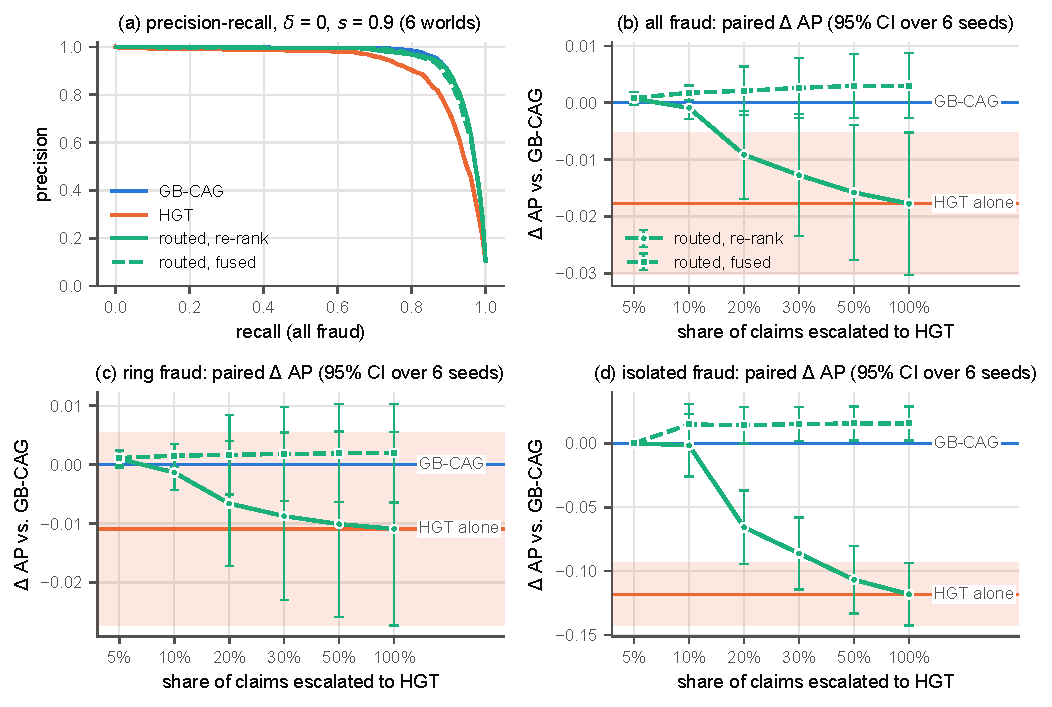
\includegraphics[width=\textwidth]{fig_cascade.pdf}
\caption{Two-stage routing from GB-CAG to HGT. (a) Precision--recall curves
for all fraud at $\delta=0$, $s=0.9$ (precision interpolated at fixed recall
and averaged over six worlds; routed systems at the escalation fraction
chosen on validation). (b)--(d) Paired difference in test AP from GB-CAG
(zero line) against the share of claims escalated, averaged over the 54
worlds, with 95\% CIs over the six seeds; orange line and band: HGT alone. The escalation fraction
actually used is chosen on validation; the curves over all fractions are
shown only to describe the trade-off.}
\label{fig:cascade}
\end{figure}

\section{Ring-volume dose-response}\label{sec:s_dose}
Table~\ref{tab:dose} gives ring AP for every method at four ring volumes (16, 8, 4 and 2 claims per ring
per month) at $\delta=0$, over seeds 1--6, whose legitimate claims, isolated fraud and ring members are
identical across volumes. The hyperparameters are those of the main experiment; the re-tuned results at
volume 4 are in Table~\MainTabLowVolume{} of the article. In a test period a ring patient files on average 9.3, 5.4, 3.7 and
3.0 claims at the four volumes, against 1.6 for other patients (95th and 99th percentiles about 3.8 and
5.2), and a ring doctor 38, 26, 20 and 18 claims against 16. At 2 claims per month a ring files about one
claim per member, rings make up 1.1\% of the non-isolated claims, and no method is far above chance. Paired
comparisons for every cell are in the repository (\texttt{results/tables/dose\_response\_comparisons.csv}).

\begin{table}[h]
\caption{Ring AP at $\delta=0$ by ring volume (claims per ring per month; 16 is the default) and structural density $s$, mean over six worlds (seeds 1--6, which share their legitimate claims across volumes), hyperparameters of the main experiment. Chance level: 0.080 at 16, 0.042 at 8, 0.021 at 4, 0.011 at 2.}\label{tab:dose}
\scriptsize
\setlength{\tabcolsep}{2pt}
\begin{tabular}{@{}lcccccccccccc@{}}
\toprule
 & \multicolumn{4}{c}{$s=0.1$} & \multicolumn{4}{c}{$s=0.5$} & \multicolumn{4}{c}{$s=0.9$} \\
\cmidrule(lr){2-5}\cmidrule(lr){6-9}\cmidrule(lr){10-13}
Method / volume & 16 & 8 & 4 & 2 & 16 & 8 & 4 & 2 & 16 & 8 & 4 & 2 \\
\midrule
GB-C & 0.084 & 0.046 & 0.024 & 0.014 & 0.086 & 0.044 & 0.023 & 0.012 & 0.087 & 0.044 & 0.022 & 0.015 \\
MLP-C & 0.088 & 0.044 & 0.024 & 0.013 & 0.087 & 0.041 & 0.024 & 0.013 & 0.095 & 0.046 & 0.024 & 0.013 \\
LR-CA & 0.923 & 0.524 & 0.106 & 0.025 & 0.888 & 0.428 & 0.087 & 0.039 & 0.868 & 0.364 & 0.088 & 0.020 \\
RF-CA & 0.875 & 0.339 & 0.057 & 0.019 & 0.838 & 0.343 & 0.064 & 0.018 & 0.844 & 0.331 & 0.064 & 0.018 \\
GB-CA & 0.925 & 0.422 & 0.049 & 0.020 & 0.905 & 0.372 & 0.052 & 0.019 & 0.889 & 0.311 & 0.055 & 0.018 \\
GB-CAG & 0.930 & 0.550 & 0.066 & 0.018 & 0.983 & 0.879 & 0.409 & 0.024 & 0.990 & 0.923 & 0.570 & 0.019 \\
\midrule
SAGE & 0.938 & 0.606 & 0.074 & 0.016 & 0.963 & 0.683 & 0.108 & 0.017 & 0.976 & 0.755 & 0.131 & 0.018 \\
RGCN & 0.933 & 0.546 & 0.066 & 0.018 & 0.953 & 0.637 & 0.112 & 0.018 & 0.954 & 0.686 & 0.142 & 0.018 \\
HAN & 0.908 & 0.469 & 0.062 & 0.014 & 0.906 & 0.507 & 0.065 & 0.018 & 0.921 & 0.520 & 0.058 & 0.014 \\
Simple-HGN & 0.915 & 0.561 & 0.074 & 0.014 & 0.960 & 0.692 & 0.133 & 0.015 & 0.957 & 0.716 & 0.151 & 0.013 \\
HGT & 0.910 & 0.544 & 0.046 & 0.016 & 0.948 & 0.649 & 0.079 & 0.017 & 0.949 & 0.689 & 0.098 & 0.016 \\
\midrule
SAGE+AG & 0.973 & 0.659 & 0.103 & 0.020 & 0.985 & 0.883 & 0.379 & 0.032 & 0.983 & 0.914 & 0.566 & 0.025 \\
HGT+AG & 0.964 & 0.546 & 0.074 & 0.019 & 0.984 & 0.872 & 0.324 & 0.024 & 0.990 & 0.916 & 0.523 & 0.023 \\
Overlap score & 0.254 & 0.141 & 0.057 & 0.018 & 0.937 & 0.721 & 0.194 & 0.030 & 0.985 & 0.866 & 0.281 & 0.029 \\
\botrule
\end{tabular}
\end{table}

\section{Confirmatory test of the hybrid result}\label{sec:s_confirm}
In seeds 1--6, after re-tuning at volume 4, SAGE+AG had higher ring AP than GB-CAG for sparse rings
($s=0.1$: 0.129 against 0.078, Holm $p=0.035$), the only significant advantage over GB-CAG in the
low-volume experiments. Because this comparison was singled out after the results had been seen, we tested
it once more as fixed in an analysis plan committed before the runs started
(\texttt{paper/hiss\_review/analysis\_plan\_round2.md}): fresh generator seeds 7--18, $\delta=0$,
$s=0.1$, volume 4, the re-tuned configurations, only GB-CAG and SAGE+AG, and one two-sided paired $t$-test
at $\alpha=0.05$. SAGE+AG had a mean ring AP of 0.129 against 0.104 for GB-CAG: a difference of $+0.024$
(95\% CI $[0.005, 0.043]$, $p=0.016$; Wilcoxon $p=0.009$), positive in nine of twelve seeds, with a
chance level of 0.021. By the pre-declared rule the advantage is confirmed; its size is about half the
exploratory estimate.

\section{Cost of training and scoring}\label{sec:s_cost}
Median training time per world (Intel Core i7-1068NG7 laptop CPU, two
threads per job with several jobs in parallel, so times are indicative) was
3~s for GB-CAG, 39~s for SAGE, 56~s for RGCN, 86~s for HAN, 126~s for HGT and
144~s for Simple-HGN; scoring a test period took at most 0.25~s for any
method. A separate single-thread benchmark on an otherwise idle machine (four
worlds at $\delta=0$) measured scoring directly. For one audit period (about
4{,}900 claims and 11{,}200 nodes), building the aggregate and graph features
took 0.05~s and the heterogeneous graph 0.01~s, and scoring every claim took
0.05~s with GB-CAG and 0.12~s with HGT. Scoring a single claim, as an online
system would, took a median of 2.1~ms (99th percentile 3.1~ms, mostly
library-call overhead) with GB-CAG on a precomputed feature row, and 10.7~ms
(14.7~ms) with HGT on the claim's exact three-hop computation subgraph (about
126 nodes, 1\% of the period graph; extraction 2.8~ms, forward pass 7.7~ms),
which reproduces the full-graph score to within $1.2\times10^{-7}$. Routing
would therefore cut the online GNN cost in proportion to the share of claims
escalated. In batch scoring the escalated claims' subgraphs overlap:
escalating 10\% of the claims already touched 55\% of the period graph, and
scoring that union took 0.08~s against 0.12~s for the whole period. None of
these figures includes keeping aggregates, graph features and degree counts
up to date as claims arrive, which an online system would need and our code
does not implement.

\section{Single-factor ablations of HGT}\label{sec:hgtarch}
Table~\ref{tab:hgt_arch} changes one factor of the tuned HGT at a time in
the same regime. Depth beyond two layers and the number of attention heads
made no significant difference (four layers $+0.002$; one, two and eight
heads $-0.037$ to $+0.013$; all Holm $p>0.5$), so there is no sign of
over-smoothing up to four layers on these graphs. Among the relations,
removing the patient--claim edges cost most ($-0.219$, Holm $p=0.005$);
removing the claim--doctor edges cost $0.113$ on rings (Holm $p=0.085$) and
$0.147$ on isolated fraud ($p<0.001$), while hospital nodes and the direct
patient--doctor relation contributed nothing measurable. The node inputs
separate the two tasks cleanly. With claim attributes set to zero, ring AP
was unchanged ($-0.012$) and isolated AP fell to chance (0.036); an HGT that
saw only the degree encodings and the graph reached a ring AP of
$0.982\pm0.018$, as high as the full model, and detected no isolated fraud.
HGT's ring detection is therefore structural---counts of who bills whom,
propagated along patient--claim--doctor paths---and its claim attributes
serve isolated fraud only. This is the information that the engineered
shared-patient features summarise directly. At default volume these counts
also carry the ring members' excess claims; Section~\MainSecLowVolume{} of the article
shows that when they do not, the GNNs fall far behind gradient boosting with
the engineered features. HGT also varied between worlds
(standard deviations up to 0.11), so with six worlds differences smaller than
about 0.05 cannot be resolved.

\begin{table}[h]
\caption{HGT single-factor ablations at $\delta=0$, $s=0.9$ (six worlds; one factor changed at a time from the tuned configuration: 3 layers, 4 heads, hidden size 32). Ring AP (mean $\pm$ s.d.), isolated AP (mean) and paired change from the full model; Holm-adjusted $p$ over every ablation comparison in this table and Table~\MainTabAblation{} of the article.}\label{tab:hgt_arch}
\scriptsize
\setlength{\tabcolsep}{2.5pt}
\begin{tabular}{@{}lcccc@{}}
\toprule
Variant & Ring AP & $\Delta$ ring AP & Isol.\ AP & $\Delta$ isol.\ AP \\
\midrule
Full model & 0.949 $\pm$ 0.052 & -- & 0.455 & -- \\
\midrule
\multicolumn{5}{@{}l}{\textit{Depth (full: 3)}} \\
1 layer & 0.788 $\pm$ 0.052 & $-0.161$ ($p=0.020$) & 0.239 & $-0.216$ ($p=0.007$) \\
2 layers & 0.947 $\pm$ 0.035 & $-0.001$ ($p=1.000$) & 0.423 & $-0.032$ ($p=1.000$) \\
4 layers & 0.951 $\pm$ 0.043 & $+0.002$ ($p=1.000$) & 0.461 & $+0.005$ ($p=1.000$) \\
\midrule
\multicolumn{5}{@{}l}{\textit{Heads (full: 4)}} \\
1 attention head & 0.920 $\pm$ 0.049 & $-0.028$ ($p=1.000$) & 0.384 & $-0.071$ ($p=0.228$) \\
2 heads & 0.911 $\pm$ 0.081 & $-0.037$ ($p=0.506$) & 0.473 & $+0.018$ ($p=0.813$) \\
8 heads & 0.961 $\pm$ 0.023 & $+0.013$ ($p=1.000$) & 0.524 & $+0.069$ ($p=0.282$) \\
\midrule
\multicolumn{5}{@{}l}{\textit{Relations}} \\
No patient--claim relation & 0.730 $\pm$ 0.055 & $-0.219$ ($p=0.005$) & 0.311 & $-0.144$ ($p=0.333$) \\
No claim--doctor relation & 0.836 $\pm$ 0.037 & $-0.113$ ($p=0.085$) & 0.308 & $-0.147$ ($p<0.001$) \\
No patient--doctor relation & 0.902 $\pm$ 0.055 & $-0.047$ ($p=0.413$) & 0.423 & $-0.032$ ($p=1.000$) \\
No hospital nodes & 0.946 $\pm$ 0.032 & $-0.002$ ($p=1.000$) & 0.427 & $-0.028$ ($p=1.000$) \\
\midrule
\multicolumn{5}{@{}l}{\textit{Node inputs}} \\
No degree encodings & 0.569 $\pm$ 0.110 & $-0.379$ ($p=0.003$) & 0.375 & $-0.080$ ($p=0.813$) \\
Claim attributes zeroed & 0.937 $\pm$ 0.064 & $-0.012$ ($p=1.000$) & 0.036 & $-0.419$ ($p<0.001$) \\
Entity attributes zeroed & 0.969 $\pm$ 0.027 & $+0.020$ ($p=1.000$) & 0.444 & $-0.011$ ($p=1.000$) \\
Degree encodings only & 0.982 $\pm$ 0.018 & $+0.033$ ($p=1.000$) & 0.040 & $-0.415$ ($p<0.001$) \\
\botrule
\end{tabular}
\end{table}

\section{Which inputs the trained models use}\label{sec:reliance}
To see which inputs the trained models use, without retraining, we permuted
one input group at a time across the test period, five times each, and
recorded the drop in ring AP: for GB-CAG the C, A and G features and each G
feature separately, and for the GNNs the claim attributes, static entity
attributes and degree encodings across nodes of each type. At $\delta=0$,
GB-CAG relied on aggregates when rings were sparse (A: $-0.80$ at $s=0.1$;
G: $-0.13$) and switched to the graph features as the block became dense (G:
$-0.81$ and $-0.88$ at $s=0.5$ and $0.9$; A: below $0.06$), above all the
normalised triadic closure of the claim ($-0.47$ on its own at $s=0.9$).
SAGE and HGT relied almost entirely on degree encodings ($-0.76$ to $-0.89$
at every density) and hardly at all on claim or entity attributes (below
$0.05$). The two kinds of score are not on a common scale: GB-CAG's measure
reliance on engineered summaries of the graph, whereas a GNN's degree
encodings are raw counts whose relational meaning is extracted by message
passing, and permutation understates groups whose information is duplicated
elsewhere. Read together with the ablations, they are consistent with both
model families detecting dense rings from the same evidence: how many
counterparties a claim's patient and doctor have, and how many of them they
share. (Full results, including isolated fraud and test-time rewiring, are in
the repository.)

\section{Figures of the mechanism ablations and of new versus recurring rings}\label{sec:s_figs}
Figs.~\ref{fig:ablation} and~\ref{fig:protocolres} show the results of Table~\MainTabAblation{} and
Table~\MainTabProtocol{} of the article with 95\% intervals.

\begin{figure}[t]
\centering
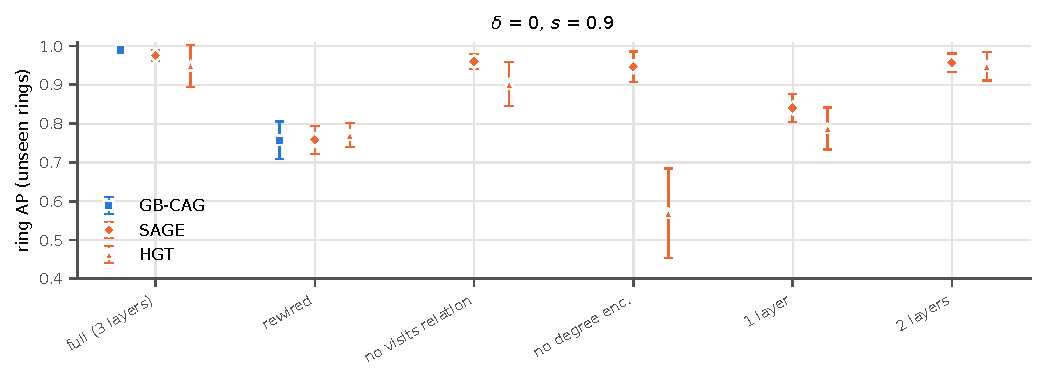
\includegraphics[width=\textwidth]{fig_ablation.pdf}
\caption{Mechanism ablations at $\delta=0$, $s=0.9$ (mean and 95\%
$t$-interval over six worlds). Rewiring preserves every node's degree but
destroys the ring block.}
\label{fig:ablation}
\end{figure}

\begin{figure}[t]
\centering
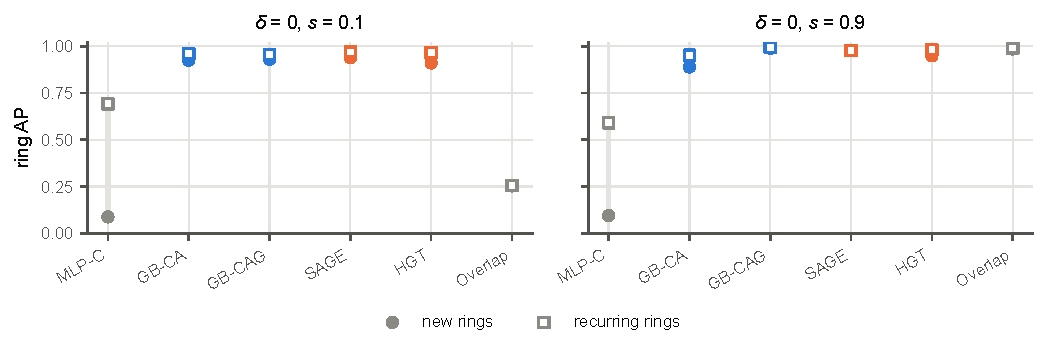
\includegraphics[width=\textwidth]{fig_protocol.pdf}
\caption{Ring AP on new versus recurring rings ($\delta=0$, six worlds).}
\label{fig:protocolres}
\end{figure}

\section{Repeated cross-validation and per-rotation tuning on the public data}\label{sec:s_kaggle}
Both analyses were specified in the plan for the second round of experiments before they were run.

\textbf{Repeated cross-validation.} The provider-disjoint five-fold rotation of the article (fold $k$ test,
fold $k+1$ validation, three training folds) was repeated with the stratified fold assignment reshuffled four more
times (seeds 1--4), giving 25 rotations with the article's split as the first. To save compute, the repetitions
covered the tabular models, the MLP and three GNNs (SAGE, HAN, HGT); RGCN, Simple-HGN and the hybrids were run on
the article's split only. Hyperparameters are those of the shared selection. Each method is compared with GB-P by
the corrected repeated cross-validation $t$-test (Nadeau and Bengio 2003; Bouckaert and Frank 2004; references
\MainRefNadeau{} and \MainRefBouckaert{} of the article), which inflates the variance
of the mean difference by $1/25 + 1/3$ instead of $1/25$, with 24 degrees of freedom, and the eight $p$-values are
Holm-adjusted. Table~\ref{tab:kaggle_repeated} shows the result. GB-P has the highest mean AP; graph features change
it by $-0.007$ and $-0.006$, with upper 95\% limits of $+0.006$ and $+0.007$; the GNNs are 0.025--0.034 lower.
No difference is significant after adjustment (smallest Holm $p=0.29$, HAN; unadjusted $p=0.036$). Without the
correction, every difference would be significant (all unadjusted $p<0.01$), which shows how strongly
overlapping training sets inflate a plain paired test.

\begin{table}[h]
\caption{Public data, five-fold rotation repeated five times (25 rotations; the first repeat is the split reported in the article): AP mean $\pm$ s.d., and the difference from GB-P with the corrected repeated cross-validation 95\% CI and Holm-adjusted $p$ (variance factor $1/25 + 1/3$, 24 degrees of freedom).}\label{tab:kaggle_repeated}
\footnotesize
\begin{tabular}{@{}lccc@{}}
\toprule
Method & AP & $\Delta$ vs.\ GB-P [95\% CI] & $p$ \\
\midrule
LR-P & 0.674 $\pm$ 0.046 & $-0.019$ [$-0.044$, $+0.006$] & 0.704 \\
RF-P & 0.674 $\pm$ 0.041 & $-0.019$ [$-0.042$, $+0.005$] & 0.704 \\
GB-P & 0.693 $\pm$ 0.045 & -- & -- \\
GB-PG & 0.686 $\pm$ 0.045 & $-0.007$ [$-0.019$, $+0.006$] & 0.704 \\
GB-PGL & 0.687 $\pm$ 0.046 & $-0.006$ [$-0.019$, $+0.007$] & 0.704 \\
MLP-P & 0.676 $\pm$ 0.042 & $-0.017$ [$-0.042$, $+0.009$] & 0.704 \\
SAGE & 0.665 $\pm$ 0.058 & $-0.028$ [$-0.066$, $+0.010$] & 0.704 \\
HAN & 0.659 $\pm$ 0.046 & $-0.034$ [$-0.066$, $-0.002$] & 0.289 \\
HGT & 0.668 $\pm$ 0.050 & $-0.025$ [$-0.055$, $+0.005$] & 0.704 \\
\botrule
\end{tabular}
\end{table}

\textbf{Per-rotation (nested) selection.} The shared selection uses a separate 60/20/20 split whose validation
providers also appear in the test folds of the rotations. Re-selecting each method's configuration inside every
rotation, from the same six candidates and on that rotation's validation fold only, removes this overlap.
Table~\ref{tab:kaggle_nested} compares nested with shared selection, and every method with GB-P when both are
selected inside each rotation. Re-selection changed AP by at most 0.010 for the tabular models and the MLP and by
$-0.008$ (HGT) to $+0.036$ (RGCN) for the GNNs and hybrids, with no change significant; SAGE selected its shared
configuration in all five rotations, and SAGE+G inherits it, so their results are identical. We had expected the
shared selection to favour the GNNs; it did not do so systematically. With every method selected inside each
rotation, GB-P remains the best method, and every GNN and hybrid is 0.023--0.053 below it (smallest Holm $p=0.051$
for SAGE and SAGE+G).

\begin{table}[h]
\caption{Public data: hyperparameters re-selected inside every rotation (nested) versus selected once on a separate split (shared; Table~\MainTabKaggle{} of the article). AP mean over the five rotations. Nested $-$ shared: change from re-selection; vs.\ nested GB-P: difference from GB-P when both are selected inside each rotation, with Holm-adjusted $p$. Intervals are corrected resampled 95\% CIs. Same choice: the shared configuration was selected in every rotation, so the results are identical. Hybrids inherit their base model's per-rotation choice.}\label{tab:kaggle_nested}
\scriptsize
\setlength{\tabcolsep}{3pt}
\begin{tabular}{@{}lcccc@{}}
\toprule
Method & Nested AP & Nested $-$ shared [95\% CI] & vs.\ nested GB-P [95\% CI] & $p$ \\
\midrule
LR-P & 0.682 & $+0.003$ [$-0.008$, $+0.015$] & $-0.024$ [$-0.055$, $+0.007$] & 0.607 \\
RF-P & 0.680 & $-0.001$ [$-0.021$, $+0.019$] & $-0.026$ [$-0.062$, $+0.010$] & 0.607 \\
GB-P & 0.706 & $+0.002$ [$-0.016$, $+0.019$] & -- & -- \\
GB-PG & 0.693 & $-0.001$ [$-0.033$, $+0.030$] & $-0.012$ [$-0.045$, $+0.020$] & 0.607 \\
GB-PGL & 0.687 & $-0.010$ [$-0.040$, $+0.020$] & $-0.019$ [$-0.057$, $+0.018$] & 0.607 \\
MLP-P & 0.688 & $+0.003$ [$-0.008$, $+0.014$] & $-0.018$ [$-0.045$, $+0.010$] & 0.607 \\
SAGE & 0.664 & same choice & $-0.042$ [$-0.062$, $-0.022$] & 0.051 \\
RGCN & 0.657 & $+0.036$ [$-0.014$, $+0.086$] & $-0.049$ [$-0.103$, $+0.005$] & 0.527 \\
HAN & 0.670 & $+0.003$ [$-0.023$, $+0.030$] & $-0.036$ [$-0.089$, $+0.017$] & 0.607 \\
Simple-HGN & 0.682 & $+0.012$ [$-0.032$, $+0.056$] & $-0.023$ [$-0.048$, $+0.001$] & 0.527 \\
HGT & 0.668 & $-0.008$ [$-0.034$, $+0.019$] & $-0.038$ [$-0.065$, $-0.011$] & 0.177 \\
SAGE+G & 0.653 & same choice & $-0.053$ [$-0.078$, $-0.027$] & 0.051 \\
HGT+G & 0.661 & $+0.013$ [$-0.018$, $+0.043$] & $-0.045$ [$-0.096$, $+0.006$] & 0.527 \\
\botrule
\end{tabular}
\end{table}

\section{Re-analysis of a small fixed benchmark}\label{sec:legacy}
To show how a small, fixed benchmark can mislead, we re-analysed one: a
synthetic dataset of 2{,}100 claims with five injected rings, produced by an
earlier, simpler generator of ours that is included in the repository,
evaluated with its own
date-sorted 60/20/20 split (Table~\ref{tab:legacy}). Such a dataset appears
to test ring detection, but this one cannot tell whether relational
structure helps, for three reasons. First, its ring claims were drawn from the
same inflated distribution as its isolated fraud, so they were anomalous on
their own: claim amount alone separates ring from legitimate claims with
ROC-AUC 0.94, more than in our most anomalous regime ($\delta=2$, 0.90), and
gradient boosting on three raw claim attributes ranks all 21 test ring claims
above every legitimate claim (ring AP 1.000). Second, the same five rings
were active for all 24 months, so every test ring claim was billed by a
doctor with labelled ring claims in training, which is the memorisation
setting of Section~\MainSecMechanism{} of the article. Third, the test split held 21 ring
claims (3--6 per ring): one claim moves ring recall by 4.8 points, even a
perfect recall has an exact 95\% interval of $[0.84, 1.00]$, so a recall gap
of a few claims between two models is within noise, and a single dataset says
nothing about variation between datasets. None of these properties is
peculiar to that dataset. A small, fixed benchmark whose injected rings
differ from legitimate claims in their features, recur across the split and
contribute a few dozen test claims cannot separate relational learning from
claim-level anomaly detection or from recognising known members. Controlling
the feature-level signal, testing on new rings and replicating worlds
removes all three confounds. Because the generator, features, evaluation unit
and tuning differ, numbers from the two set-ups are not directly comparable.

\begin{table}[h]
\caption{A small fixed benchmark (2,100 claims, five rings; an earlier, simpler generator of ours, included in the repository), re-analysed with its own split (date-sorted, 60/20/20), compared with our benchmark. Benchmark ranges span $\delta=0$ to $\delta=2$ ($s=0.5$, six worlds each; ring AP and recall of GB-C pooled over $s$). Shift and ROC-AUC use raw claim amounts, not adjusted for specialty, for both. Interval: exact 95\% binomial.}\label{tab:legacy}
\scriptsize
\begin{tabular}{@{}p{5.0cm}p{3.1cm}p{3.6cm}@{}}
\toprule
 & Fixed dataset & This benchmark \\
\midrule
Claims in total (in the test split / period) & 2,100 (420) & 20,176 (4,924), mean per world \\
Ring claims in test & 21 (3--6 per ring) & 384 (4 rings $\times$ 96) \\
Rings & 5, active all 24 months & 4 per period, each active 6 months \\
Test-ring doctors with labelled ring claims in training & 100\% & 0\% (by design) \\
Ring vs.\ legitimate log-amount shift (s.d.) & 1.49 & 0.11 ($\delta=0$) to 1.87 ($\delta=2$) \\
ROC-AUC of claim amount alone, ring vs.\ legitimate & 0.94 & 0.53 to 0.90 \\
Ring AP, GB on claim attributes only & 1.000 & 0.086 to 0.811 \\
Ring recall, GB on claim attributes only & 21/21 [0.84, 1.00] & 0.15 to 0.76 \\
Generated datasets (independent generator seeds) & 1 (1) & 54 (6) \\
\botrule
\end{tabular}
\end{table}

\end{document}
